
\subsection{Messaging}


\subsection{Create User Profile}


In order for an IMP identity to request a relationship with the administration portal, the portal has to provide a relationship template to the IMP client of the user. The template can be made accessible to the IMP client trough a new web page which displays the template ID as QR code if the user is logged in. Each time a logged in user requests the web page, the web server requests the IMP connector to create a relationship template.

The IMP connector provides an API for creation of relationship templates as part of its REST interface. Through a HTTP POST call, the web server transmits the appropriate request to the connector and receives the template as response. The web page of the administration portal can then render the template as a QR code on the web page.

\begin{figure}[h]
    \centering
    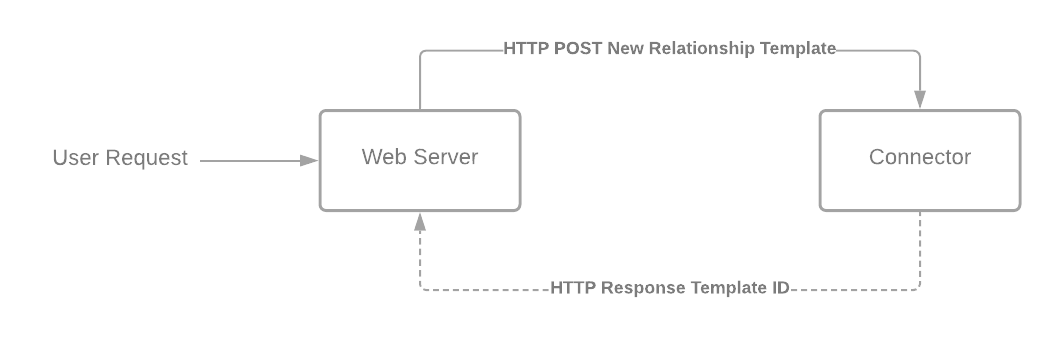
\includegraphics[scale=0.3]{Diagrams/Integration Architecture 1/Overview/Relationship Template REST.png}
\end{figure}

This is one example, where the OZG system could use the REST interface for integration with the IMP system. However, messaging can improve the integration solution to be more maintainable, stable and scalable and will be the preferred option in following scenarios. Using messaging, the web server can publish a message containing the request for a new relationship template on a "Relationship Template Request" channel, where the connector receives it, creates the template and publishes a reply message containing the template ID on the "Relationship Template Reply" channel.

\begin{figure}[h]
    \centering
    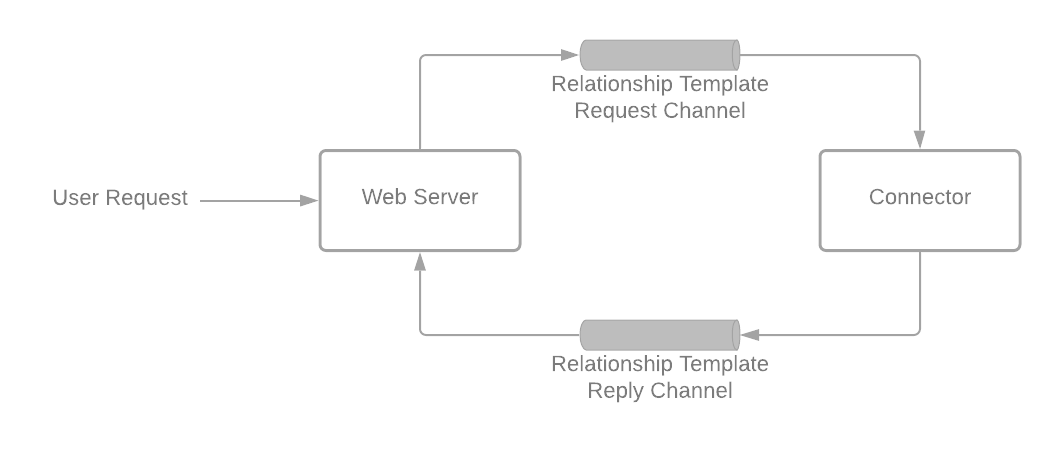
\includegraphics[scale=0.3]{Diagrams/Integration Architecture 1/Overview/Relationship Template Messaging.png}
\end{figure}

It could happen, that in future, the API of the connector changes. If the web server integrated the connector through its REST interface, this would require the request code of the web server to be changed. If messaging is used, messages leaving the "Relationship Template Request" channel could be mapped to the new API signature through an additional messaging component called message translator. This is an example for how a messaging can improve maintainability of an integration architecture.

\begin{figure}[h]
    \centering
    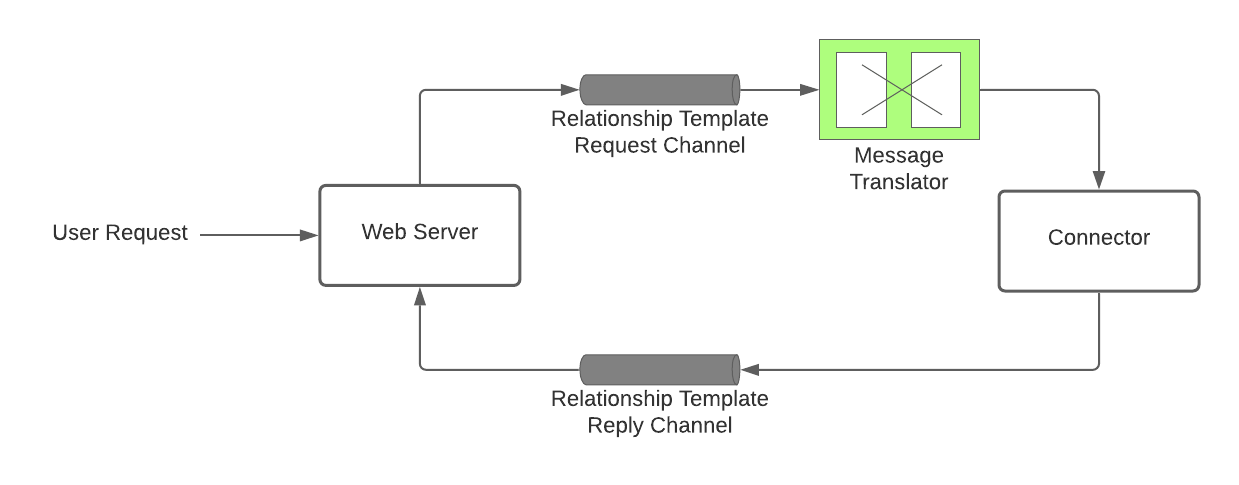
\includegraphics[scale=0.3]{Diagrams/Integration Architecture 1/Overview/Relationship Template Messaging Improved.png}
\end{figure}


When the user is presented with the web page containing the QR code, the user can scan it with its IMP client. Based on the template ID, the client retrieves the template from the IMP server and displays it for the user. If the user accepts the template, the client sends a relationship request to the IMP server, who forwards it to the corresponding connector.

Upon receiving the request, the connector has to notify the administration portal of an incoming relationship request. If the web server does not provide an HTTP endpoint for communicating with the connector, it won't be able to receive a notification about the arrival of a new relationship request. The server would have to regularly request a status update which is not efficient. Using messaging, the connector can publish the content of the relationship request to a "Relationship Request" channel where the subscribed administration portal will be notified. The administration portal can process the relationship request and publish a message containing a response on the "Relationship Response" channel, where the connector will be notified. Through the IMP server, the response server is routed to the IMP client and the relationship is established.
In order to map relationships to user profiles, the administration portal manages a database which contains entries consisting of IMP identity ID, relationship ID and user profile ID.

\begin{figure}[h]
    \centering
    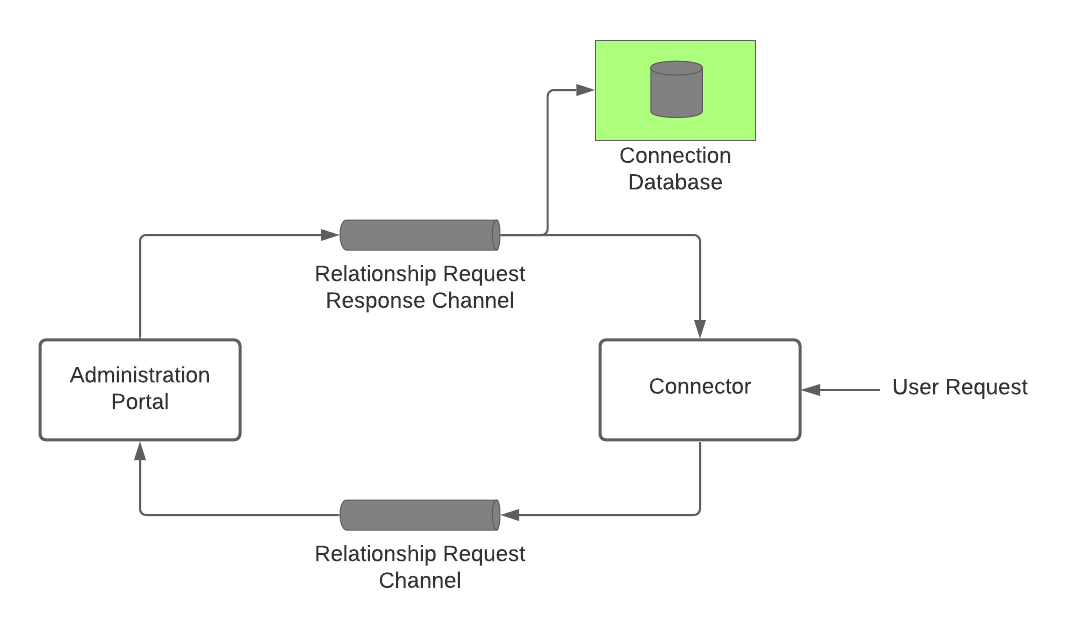
\includegraphics[scale=0.3]{Diagrams/Integration Architecture 1/Overview/Relationship Request.png}
\end{figure}

\subsection{Attribute Synchronization}

As administration portal and IMP identity established a relationship, the connector can be excluded from the diagram for better visualisation. Behind the scenes, all interactions between administration portal and IMP client still go through connector and IMP server.

If the user requests the change of a shared attribute through the IMP client, it sends an attribute change request to the administration portal by publishing a message on the "Inbound Attribute Change Request" channel. After the administration portal decides to accept the request, it can publish a message to the "Outbound Attribute Change Response" channel. This message will on one hand be received by the IMP client and on the other hand result in an update of the user profile. 

\begin{figure}[h]
    \centering
    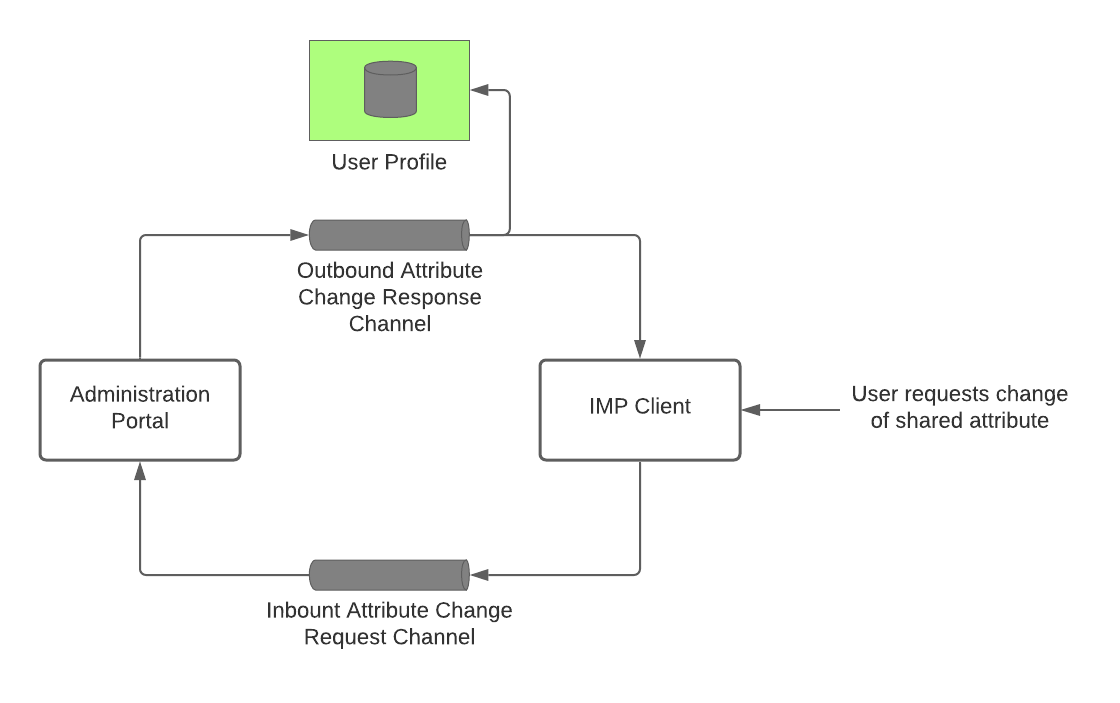
\includegraphics[scale=0.3]{Diagrams/Integration Architecture 1/Overview/Attribute Change IMP Client.png}
\end{figure}

If the user requests the change of a shared attribute through the web page of the administration portal, the web server sends an attribute change request to the "Outbound Attribute Change Request" channel which is received by the IMP client. If the user accepts the request, the client publishes a message on the "Inbound Attribute Change Response" channel where it results in an update of the user profile.

\begin{figure}[h]
    \centering
    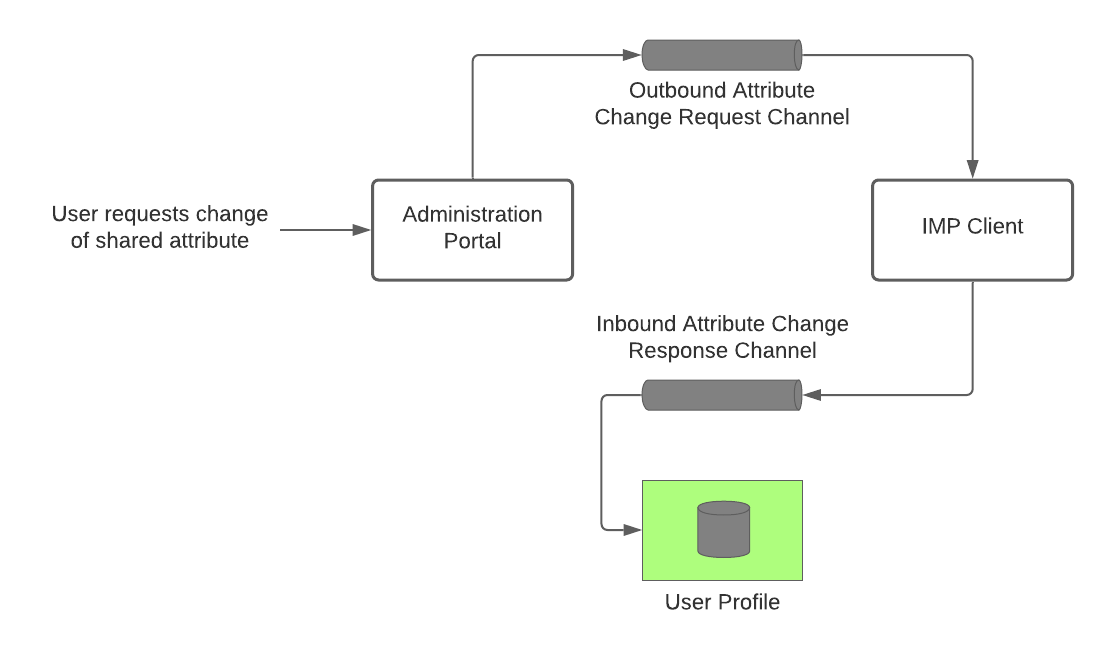
\includegraphics[scale=0.3]{Diagrams/Integration Architecture 1/Overview/Attribute Change Web Page.png}
\end{figure}

\subsection{Login to a User Profile}

\begin{figure}[h]
    \centering
    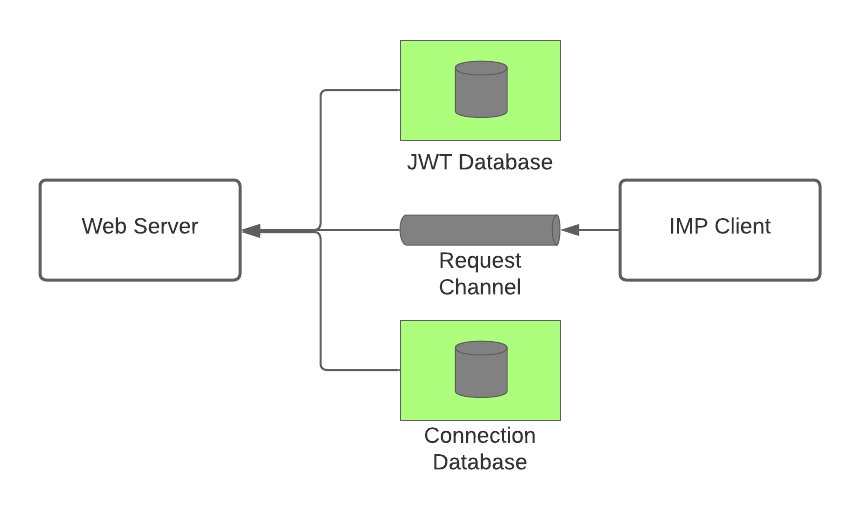
\includegraphics[scale=0.3]{Diagrams/Integration Architecture 1/Overview/Login.png}
\end{figure}

\subsection{Communication}